\chapter{Polinomios y fracciones algebraicas}

\begin{tikzpicture}
	\fill [left color=red!50, right color=teal!50] (0,0) rectangle (6.5,.2);
	\fill [left color=teal!50, right color=blue!50] (6.5,0) rectangle (11.5,.2);
	\end{tikzpicture}
	
	
\vspace{15mm}


\begin{adjustwidth}{40pt}{40pt}
\begin{cuadro-gris}

	\begin{multicols}{2}
	$\triangleright \quad$ Polinomios. Operaciones.
	
	$\triangleright \quad$ Regla de Ruffini y teorema del resto.
	
	$\triangleright \quad$ Factorización de polinomios.
	
	$\triangleright \quad$ Fracciones algebráicas.
	\end{multicols}
	
\end{cuadro-gris}
\end{adjustwidth}


\vspace{1cm}

\begin{myexampleblock}{Aritmética vs Álgebra}
\vspace{2mm} \textbf{Aritmética}: realmente es algo que se utiliza a diario sin darse cuenta, incluye todo lo relacionado a números. La palabra aritmética desciende de un término griego (aritmo) el cual significa número. Es una rama básica de las matemáticas y con ésta se trabaja tradicionalmente con las 4 operaciones básicas que solemos utilizar: resta, suma, división y multiplicación. También existe una aritmética avanzada o superior, conocida como \emph{teoría de números}.


\vspace{2mm} \textbf{Álgebra}: también es una rama perteneciente a las matemáticas; la palabra  derivad de un término árabe (al-Jabr), fueron quienes más contribuyeron a la formación de esta rama; al-Jabr realmente era un término médico que significaba algo así como poner en orden las piezas rotas; los árabes inventaron el álgebra con el fin de poder razonar con lógica, donde lo importante era el razonamiento y no los valores, debido a esto tenía letras y no números, puesto que lo que buscaban era poder razonar sin importar las cifras. Dentro de las matemáticas podemos poner al álgebra como en un segundo nivel seguido de la aritmética. Lo que la diferencia principalmente de la aritmética es que no trabaja solo con números, sino que mezcla estos con otros valores que son desconocidos (incógnitas o variables).

\vspace{2mm} \textcolor{gris}{Fuente: https://educar.doncomos.com/saber-diferenciar-algebra-aritmetica}	

\end{myexampleblock}


\begin{figure}[H]
	\centering
	
\includegraphics[width=0.5\textwidth]{img-pol/pol02.png}
\end{figure}



\vspace{1cm}
\section{Polinomios}

\begin{tikzpicture}
	\fill [left color=red!50, right color=teal!50] (0,0) rectangle (3.5,.1);
	\fill [left color=teal!50, right color=blue!50] (3.5,0) rectangle (7.5,.1);
	\end{tikzpicture}
\vspace{0.5cm}


Un \textbf{monomio} es una expresión algebraica formada por un número (\emph{coeficiente}) y una o varias letras (variables) elevadas a exponentes naturales (\emph{parte literal}).

Se llama \text{grado del monomio} al exponente de la parte literal (si es de una sola variable) o la suma de los exponentes (si el monomio es de varias variables).

Dos momonios son \emph{semejantes} si tienen la misma parte literal.

\vspace{5mm}
\begin{definition}[ Polinomio]

Un \textbf{polinomio} de una variable es una expresión del tipo:

$$\boldsymbol{ p(x)\ = \ a_0x^n+a_1x^{n-1}+\cdots +a_{n-2}x^2+a_{n-1}x+a_0 }$$	

$a_i: \ i=0,1,2,\cdots n \ $ son los coeficientes.

\end{definition}

\vspace{3mm}
\begin{definition}

\vspace{2mm}\textbf{Grado de un polinomio} es el exponente de la máxima potencia de la variable (el mayor grado de los monomios que forman el polinomio).
Cada uno de los monomios que forman el polinomio recibe el nombre de \textbf{término}. Los polinomios de dos términos se llaman \emph{binomios}, los de tres \emph{trinomios}.
\end{definition}


\vspace{3mm}
\begin{definition}[ Valor numérico de un polinomio]

\textbf{Valor numérico} del polinomio $\ p(x) \ $ en $\ x=a\in \mathbb R\ $ es el número que resulta al sustituir en el polinomio $x$ por $a$, es decir, calcular $\ p(a)$.	
\end{definition}

\vspace{5mm}

\begin{miejemplo}

El grado de $\ -3x^4\ $ es $\ 4$, el de $\ 23x^3y^2z \ $ es $\ 6=3+2+1$.

\vspace{2mm} Si $p(x)=x^4+7x+1 \ \to \ $ el valor numérico en $x=-2$ es $\ p(-2)=(-2)^4+7\, (-2)+1=3$. El grado de $p(x)$ es $4$.
\end{miejemplo}

\vspace{1cm}
\section{Operaciones con polinomios}

\begin{tikzpicture}
	\fill [left color=red!50, right color=teal!50] (0,0) rectangle (3.5,.1);
	\fill [left color=teal!50, right color=blue!50] (3.5,0) rectangle (7.5,.1);
	\end{tikzpicture}

\vspace{0.5cm}


\begin{figure}[H]
	\centering
	\includegraphics[width=0.5\textwidth]{img-pol/pol03.png}
\end{figure}



\vspace{0.75cm}

\subsection{Suma y producto de polinomios}

\begin{tikzpicture}
	\fill [left color=red!50, right color=teal!50] (0,0) rectangle (3.5,.01);
	\fill [left color=teal!50, right color=blue!50] (3.5,0) rectangle (7.5,.01);
	\end{tikzpicture}
\vspace{0.5cm}

$\triangleright \qquad 3(3x^3-4x+1)-2(4x^2-5x)=9x^3-12x+3-8x^2+10x=9x^3-8x^2-2x+3$

$\triangleright \qquad (2x^2+1)\cdot (3x^3-2x+5)=6x^4-4x^3+10x^2+3x^2-2x+5=6x^4-4x^3+13x^2-2x+5$

\begin{itemize}
\item El producto de un número $k$ por un polinomio $p(x)$ es el polinomio $k\, p(x)$ en que todos los coeficientes de $p(x)$ se han multiplicado por $k$.
\item La suma de polinomios verifica las propiedades \emph{conmutativa} \textcolor{gris}{$[ \ p(x)+q(x)=q(x)+p(x) \ ]$} y \emph{asociativa} \textcolor{gris}{$[ \ p(x)+(q(x)+r(x))=(p(x)+q(x))+r(x) \ ]$}. El neutro para la suma es el polinomio nulo, $0$. El \emph{opuesto} a un polinomio $p(x)$ es el polinomio $-p(x)$, en que todos los coeficientes han cambiado de signo, de ese modo, $p(x)-q(x)=p(x)+(-q(x))$.
\item El producto de polinomios verifica las propiedades \emph{conmutativa} \textcolor{gris}{$[ \ p(x)\cdot q(x)=q(x) \cdot p(x) \ ]$} y \emph{asociativa} \textcolor{gris}{$[ \ p(x)\,(q(x)\, r(x))=(p(x)\ q(x))\, r(x) \ ]$}. El neutro para el producto es el polinomio unidad, $1$. El producto de polinomios no tiene \emph{inverso}.
\item Se cumple la propiedad \emph{distribituva} del producto respecto de la suma: $\ p(x)\, (q(x)+r(x))=p(x)\, q(x)+p(x)\, r(x)$. Esta  propiedad, leída de derecha a izquierda, es la que permite sacar \emph{factor común}.
\end{itemize}



\subsection{Productos notables}

\begin{tikzpicture}
	\fill [left color=red!50, right color=teal!50] (0,0) rectangle (3.5,.01);
	\fill [left color=teal!50, right color=blue!50] (3.5,0) rectangle (7.5,.01);
	\end{tikzpicture}
\vspace{0.5cm}

Son casos particulares del binomio de Newton que, por la frecuencia con que aparecen, vale la pena recordar.

$$ \boldsymbol{ \boxed{ \ \subrayado{ \ (a\pm b)^2 \ = \ a^2 \pm 2ab+b^2  \ } \ } \ ;\qquad \qquad \boxed{ \ \subrayado{ \ (a+b) \, (a-b) \ = \ a^2-b^2} \ } \ } $$

\color{gris}

$$(a\pm b)^3 \ = \ a^3\pm 3a^2b\pm 3ab^2+b^3\, ; \qquad \qquad a^3\pm b^3 \ = \  (a\pm b)\, (a^2\mp ab+b^3)$$

$$(a+b+c)^2 \ = \ a^2+b^2+c^2 \, + \, 2ab \, + \, 2ac \, + \, 2bc$$

\color{black}

\begin{figure}[H]
	\centering
	
\includegraphics[width=0.35\textwidth]{img-pol/pol04.png}
\end{figure}

\subsection{División de polinomios}

\begin{tikzpicture}
	\fill [left color=red!50, right color=teal!50] (0,0) rectangle (3.5,.01);
	\fill [left color=teal!50, right color=blue!50] (3.5,0) rectangle (7.5,.01);
	\end{tikzpicture}
\vspace{0.5cm}



% Please add the following required packages to your document preamble:
% \usepackage{multirow}
\begin{table}[H]
\centering
\begin{tabular}{llllll}
\multicolumn{1}{l|}{$D(x)$} & $\ d(x)\ $ & $\qquad$ & \multirow{2}{*}{$D(x)=d(x)\, c(x)+r(x)$} & $\qquad$ & \multirow{2}{*}{$\dfrac{D(x)}{d(x)}=c(x)+\dfrac{r(x)}{d(x)}$} \\ \cline{2-2}
$r(x)$ & $\ c(x)\ $ &  &  &  & 
\end{tabular}
\end{table}

\begin{itemize}
\item Para efectuar la división, grado $D(x) \geq $ grado $d(x)$	
\item Si $r(x)=0 \ \to \ $ la división es exacta.
\item La división acaba al obtener grado $r(x) \leq $ grado $d(x)$
\end{itemize}

\vspace{5mm}
Recordemos como efectuamos la división entre números.

\underline{División numérica}:
\begin{table}[H]
\centering
\small
\begin{tabular}{llrrrrl}
\textcolor{gris}{$183\, :\, 27 \to \textcolor{red}{6}\cdots $} &  & 1 & 8 & 3 & \multicolumn{1}{r|}{4} & $\quad 27$ \\ \cline{7-7} 
\textcolor{gris}{$6\cdot 27$} & \scriptsize{\textcolor{gris}{$\overrightarrow{\text{su opuesto}} \qquad$}} & \textcolor{gris}{-1} & \textcolor{gris}{6} & \textcolor{gris}{2} &  & $\quad \textcolor{red}{6}\, \textcolor{blue}{7}$ \\ \cline{3-5}
\textcolor{gris}{$214\, : \, 27 \to \textcolor{blue}{7}\cdots$} &  &  & 2 & 1 & 4 &  \\
\textcolor{gris}{$7\cdot 27$} & \scriptsize{\textcolor{gris}{$\overrightarrow{\text{su opuesto}} \qquad$}} &  & \textcolor{gris}{-1} & \textcolor{gris}{8} & \textcolor{gris}{9} &  \\ \cline{5-6}
 &  &  &  & 2 & 5 & 
\end{tabular}
\end{table}

Del mismo modo, para dividir polinomios el procedimiento es:

\underline{División de polinomios}:
\begin{table}[H]
\centering
\begin{tabular}{llrrrrrll}
\textcolor{gris}{$6x^2\ :\ 2x^2= \textcolor{red}{3x^2}$} &  & $6x^4$ & $+5x^3$ & $+x^2$ & $+3x$ & $-2$ & \multicolumn{1}{l|}{$\quad$} & $2x^2-x+3$ \\ \cline{9-9} 
\textcolor{gris}{$3x^2\, (2x^2-x+3)$} & \scriptsize{\textcolor{gris}{$\overrightarrow{\text{su opuesto}} \qquad$}} & $-6x^4$ & $+3x^3$ & $-9x^2$ &  &  &  & $\textcolor{red}{3x^2}\, + \, \textcolor{blue}{4x}\, -\, \textcolor{DarkGreen}{2}$ \\ \cline{3-5}
\textcolor{gris}{$8x^3\ : \ 2x^2=\textcolor{blue}{4x}$} &  &  & $8x^3$ & $-8x^2$ & $+3x$ & $-2$ &  &  \\
\textcolor{gris}{$4x\, (2x^2-x+3)$} & \scriptsize{\textcolor{gris}{$\overrightarrow{\text{su opuesto}}$}} &  & $-8x^3$ & $+4x^2$ & $-12x$ &  &  &  \\ \cline{4-6}
\textcolor{gris}{$-4x^2 \  : \ 2x^2=\textcolor{DarkGreen}{-2}$} &  &  &  & $-4x^2$ & $-9x$ & $-2$ &  &  \\
\textcolor{gris}{$-2\, (2x^2-x+3)$} & \scriptsize{\textcolor{gris}{$\overrightarrow{\text{su opuesto}}$}} &  &  & $4x^2$ & $-2x$ & $+6$ &  &  \\ \cline{5-7}
 &  &  &  &  & $-11x$ & $+4$ &  & 
\end{tabular}
\end{table}

\vspace{5mm}

%%%%%
\begin{miejercicio}

Calcula: $\quad (2x+1)(3x-2)(5x-1)$

\vspace{-2mm}
\rule{250pt}{0.1pt}	

$(2x+1)(3x-2)(5x-1)=((2x+1)(3x-2))\, (5x-1)= (6x-4x^2+3-2x)(5x-1)=(-4x^2+4x+3)(5x-1)=-20x^3+20x^2+15x+4x^2-4x-3=-20x^3+24x^2+11x-3$
\end{miejercicio}

%%%%% 
\vspace{5mm}
\begin{miejercicio}

Extrae factor común: $\quad 28x^5-12x^4+16x^3$

\vspace{-2mm}
\rule{250pt}{0.1pt}	

$28x^5-12x^4+16x^3=4x^3\, (7x^2-3x+4)$
\end{miejercicio}

%%%%%
\vspace{5mm}
\begin{miejercicio}

Calcula: $\quad a)\ \left( \dfrac{2x}{3}-\dfrac{3}{2} \right)^2 ; \qquad b)\ (3x+4)(3x-4)\, ; \qquad c)\ (-3x-2)(-3x+2)$

\vspace{-2mm}


\rule{250pt}{0.1pt}	

\vspace{2mm} $\triangleright \quad  a)\ \left( \dfrac{2x}{3}-\dfrac{3}{2} \right)^2 =\left( \dfrac{3x}{2} \right)^2 - 2 \, \dfrac{3x}{2} \, \dfrac{2}{3} + \left( \dfrac{2}{3} \right)^2=\dfrac{4x^2}{9}-2x+\dfrac{9}{4} $


\vspace{2mm} $\triangleright \quad b)\ (3x+4)(3x-4) = (3x)^2-4^2=9x^2-16$


\vspace{2mm} $\triangleright \quad c)\ (-3x-2)(-3x+2)=-(3x+2)(3x-2)=-(9x^2-4)=4-9x^2 $
\end{miejercicio}

%%%%%
\vspace{5mm}
\begin{miejercicio}

Calcula: $\quad (3x^3-2x^2+5)\, : \, (2x^2-x+1) \quad$  Comprueba el resultado.

\vspace{-2mm}
\rule{250pt}{0.1pt}	

\begin{table}[H]
\centering
\begin{tabular}{rrrrll}
$3x^3$ & $-2x^2$ &  & $+5$ & \multicolumn{1}{l|}{$\quad$} & $2x^2-x+1$ \\ \cline{6-6} \\
$-3x^3$ & $+\dfrac 3 2 x^2$ & $-\dfrac 3 2 x$ &  &  & $\dfrac 3 2 x -\dfrac 1 4$ \\  \\ \cline{1-3} \\ 
 & $-\dfrac 1 2 x^2$ & $-\dfrac 3 2 x$ & $+5$ &  &  \\
 & $\dfrac 1 2 x^2$ & $-\dfrac 1 4 x$ & $+\dfrac 1 4 $ &  &  \\ \\ \cline{2-4} \\
 &  & $-\dfrac 7 4 x$ & $+\dfrac{21}{4}$ &  & 
\end{tabular}
\end{table}


Prueba de la división: $\quad (2x^2-x+1)\left( \dfrac 3 2 x-\dfrac 1 4 \right) \, + \, \left( -\dfrac 7 4 x + \dfrac{21}4 \right)=$

$=\left( 3x^3-\dfrac 1 2 x^2 -\dfrac 3 2 x^2 +\dfrac 1 4 x + \dfrac 3 2 x-\dfrac 1 4 \right) \, + \, \left( -\dfrac 7 x x + \dfrac{21}4 \right)=$

$=\left( 3x^3-2x^2+\dfrac 7 4 x -\dfrac 1 4 \right) \, + \, \left( -\dfrac 7 x x + \dfrac{21}4 \right) \ = \ 3x^3-2x^2+5$ \textcolor{gris}{\QED}

\vspace{5mm} $ \dfrac{(3x^3-2x^2+5)}{(2x^2-x+1) } \ = \ \left( \dfrac 3 2 x -\dfrac 1 4  \right) \, (2x^2-x+1) \ + \ \left( -\dfrac 7 4 x +\dfrac {21}4 \right)$

\end{miejercicio}

%%%%%
\begin{miejercicio}

Encuentra dos polinomios tales que al dividirlos el cociente sea $p(x)=x^2-x-3$ y el resto $q(x)=-3x^2-1$.

\vspace{-2mm}
\rule{250pt}{0.1pt}	

Sean $A(x)$ y $B(x)$ los polinomios buscados, por la prueba de la división, $A(x)=B(x)\, p(x) \, + \, q(x)$

\vspace{2mm} La respuesta es infinita, para cualquier $B(x)$ que nos inventemos, obtenemos el $A(x)$ correspondiente. Como pasa con los números \textcolor{gris}{$\quad  \dfrac 3 2 ; \, \dfrac {4}{3}; \,  \dfrac{-8}{-7} ; \, \cdots $ todos tienen el mismo cociente $1$ y el mismo resto $1$, $D=d(1)+(1) \ \forall d \, \exists D$}.

\vspace{2mm} Eso sí, al ser el resto un polinomio de orden 2, el divisor ha de ser un polinomio de tercer grado o superior.

\vspace{2mm} Aplicando la prueba de la división, $A=B\, p+q$ obtenemos, para cada $B$ el $A$ correspondiente.

\vspace{2mm} Por ejemplo, para $B=x^3-2$, se obtiene $A(x)=(x^3-2)(x^2-x-3)+(-3x^2-1)=x^5-x^4-3x^3-5x^2+2x+5$
\end{miejercicio}




\section{Regla de Ruffini. Teorema del resto}

\begin{tikzpicture}
	\fill [left color=red!50, right color=teal!50] (0,0) rectangle (3.5,.1);
	\fill [left color=teal!50, right color=blue!50] (3.5,0) rectangle (7.5,.1);
	\end{tikzpicture}
\vspace{0.5cm}

El método de Ruffini es un algoritmo muy útil en las divisiones de polinomios en que el denominador sea un polinomio del tipo $\boldsymbol{x-a}$

\vspace{5mm}
\begin{multicols}{2}
\begin{table}[H]
\centering
\begin{tabular}{rrrrr}
$2x^3$ & \textcolor{DarkGreen}{$-3x^2$} & $-5x$ & \multicolumn{1}{r|}{$+7$} & \textcolor{Brown}{$ x-2 \quad $} \\ \cline{5-5} 
$-2x^3$ & \textcolor{DarkGreen}{$+4x^2$} &  &  & \textcolor{red}{$2x^2+x-3$} \\ \cline{1-2}
 & $x^2$ & \textcolor{DarkGreen}{$-5x$} & $+7$ &  \\
 & $-x^2$ & \textcolor{DarkGreen}{$+2x$} &  &  \\ \cline{2-3}
 &  & $-3x$ & \textcolor{DarkGreen}{$+7$} &  \\
 &  & $3x$ & \textcolor{DarkGreen}{$-6$} &  \\ \cline{3-4}
 &  &  & \textcolor{NavyBlue}{$1$} & 
\end{tabular}
\end{table}
\begin{center}\textbf{\underline{Regla de Ruffini}}: \end{center}
	
\begin{table}[H]
\centering
\begin{tabular}{rrrrr}
 & \textcolor{gris}{$2x^3$} & \textcolor{gris}{$-3x^2$} & \textcolor{gris}{$-5x$} & \textcolor{gris}{$+7$} \\
\multicolumn{1}{r|}{\textcolor{gris}{$x-\boxed{2}$}} & 2 & \textcolor{DarkGreen}{-3} & \textcolor{DarkGreen}{-5} & \textcolor{DarkGreen}{7} \\
\multicolumn{1}{r|}{\textcolor{Brown}{2}} &  & \textcolor{DarkGreen}{4} & \textcolor{DarkGreen}{2} & \textcolor{DarkGreen}{-6} \\ \hline
\multicolumn{1}{r|}{} & \textcolor{red}{2} & \textcolor{red}{1} & \multicolumn{1}{r|}{\textcolor{red}{-3}} & \textcolor{NavyBlue}{1} \\ \cline{5-5} 
 & \textcolor{gris}{$2x^2$} & \textcolor{gris}{$+x$} & \textcolor{gris}{$-3$} & 
\end{tabular}
\end{table}
\end{multicols}

Se escriben los coeficientes del polinomio dividendo completo y ordenado, \textbf{si falta algún término hay que poner un cero}. Se hace la cruz típica del método de Ruffini y se coloca el $a$ del polinomio divisor $x-2$ a la izquierda de la cruz, en este caso \textcolor{Brown}{2}.

Bajamos el primer coeficiente del polinomio dividendo, \textcolor{red}{$2$} y multiplicamos por \textcolor{Brown}{2}, el resultado, 	\textcolor{DarkGreen}{4} se coloca debajo del segundo coeficiente del dividendo y se suma, -3+\textcolor{DarkGreen}{4}=\textcolor{Red}{1}. Se procede del mismo moda hasta acabar.

Como el divisor es de primer grado, el cociente será un de grado menos que el dividendo, sus coeficientes aparecen en la última fila en rojo. El resto de la división será un polinomio de orden cero, un número; aparece en azul.

\begin{table}[H]
\centering
\begin{tabular}{llccccl}
 &  &  & $\boxed{2\times 2=\textcolor{red}{4}}$ & $\boxed{1\times 2=\textcolor{red}{2}}$ & $\boxed{-3\times 2=\textcolor{red}{-6}}$ & \multicolumn{1}{c}{} \\ \\
 & \multicolumn{1}{l|}{} & $\quad 2$ & -3 & -5 & 7 &  \\
$a$  del divisor $x-a$ & \multicolumn{1}{l|}{$\quad 2$} & $\quad \downarrow$ & \textcolor{red}{4} & \textcolor{red}{2} & \textcolor{red}{-6} &  \\ \cline{2-6}
coeficientes del cociente & \multicolumn{1}{l|}{} & $\quad 2$ & \textcolor{blue}{1} & \multicolumn{1}{c|}{\textcolor{blue}{-3}} & \textcolor{blue}{1} & Resto \\ \cline{6-6} \\
 &  &  & $\boxed{-3+4=\textcolor{blue}{1}}$ & $\boxed{-5+2=\textcolor{blue}{-3}}$ & $\boxed{7-6=\textcolor{blue}{1}}$ & \multicolumn{1}{c}{}
\end{tabular}
\end{table}


\vspace{5mm}
\begin{miejemplo}

Divide: $\quad (3x^4-30x^2-7x+2) 	\,  :\, (x+3) $

\begin{table}[H]
\centering
\begin{tabular}{rrrrrr}
 & \textcolor{gris}{$3x^4$} &  & \textcolor{gris}{$-30x^2$} & \textcolor{gris}{$-7x$} & \textcolor{gris}{$+2$} \\
\multicolumn{1}{r|}{\textcolor{gris}{$x-\boxed{-3}$}} & 3 & \textbf{0} & -30 & -7 & 2 \\
\multicolumn{1}{r|}{-3} &  & -9 & 27 & 9 & -6 \\ \hline
\multicolumn{1}{r|}{} & 3 & -9 & -3 & \multicolumn{1}{r|}{2} & -4 \\ \cline{6-6} 
 & \textcolor{gris}{$3x^3$} & \textcolor{gris}{$-9x^2$} & \textcolor{gris}{$-3x$} & \textcolor{gris}{$+2$} & 
\end{tabular}
\end{table}
Cociente: $\ 3x^3-9x^2-3x+2\, ; \ $ resto: $\ -4$ 

\vspace{2mm} Nótese el \emph{cero} que hemos colocado como coeficiente de $x^3$ en la fila de Ruffini.
\end{miejemplo}

\vspace{5mm}

\begin{miejercicio}

Realiza las divisiones siguientes:
\hspace{1.1cm} $a)\ \ (3x^4-5x^3-8x^2-5) \, : \, (x-3)\, ;$

\vspace{2mm}$b) \ \ (4x^3-2x+3)\, : \, (x+1)	\, ;\quad  \qquad \qquad c)\ \ (5x^3+7x^2+3x-5)\, : \, (2x+1)$

\rule{250pt}{0.1pt}

\begin{multicols}{2}
a)
\begin{table}[H]
\centering
\begin{tabular}{r|rrrrr}
 & 3 & 5 & -8 & 0 & 5 \\
3 &  & 9 & 12 & 12 & 36 \\ \hline
 & 3 & 4 & 4 & \multicolumn{1}{r|}{12} & 31 \\ \cline{6-6} 
\end{tabular}
\end{table}
Cociente: $\ 3x^3+4x^4+4x+12\, ; \ $ 

Resto: $\ 31$

b)
\begin{table}[H]
\centering
\begin{tabular}{r|rrrr}
 & 4 & 0 & -2 & 3 \\
-1 &  & -4 & 4 & -2 \\ \hline
 & 4 & -4 & \multicolumn{1}{r|}{2} & 1 \\ \cline{5-5} 
\end{tabular}
\end{table}
Cociente: $\ 4x^2+4x+2\, ; \ $ 

Resto: $\ 1$	
\end{multicols}

\vspace{5mm}
La última división, apartado $c)$, no se puede hacer por Ruffini ya que el denominador no es de la forma $x-a$. Por ello habría que hacerla por el método tradicional; a no ser que agudicemos la astucia y convirtamos el polinomio divisor en uno de la forma $x-a$:

c) \vspace{2mm} \begin{small} $\dfrac{5x^3+7x^2+3x-5}{2x+1} = \dfrac{5x^3+7x^2+3x-5}{2(x+\frac 1 2)}  = \dfrac{ \dfrac{5x^3+7x^2+3x-5}{2} }{x+\frac 1 2}=\dfrac{\frac 5 2 x^3+\frac 7 2 x^2+\frac 3 2 x-\frac 5 2}{x+\frac 1 2}  $\end{small}

\vspace{2mm} --- División tradicional:
\begin{table}[H]
\centering
\begin{tabular}{rrrrc}
$5x^3$ & $+7x^2$ & $+3x$ & \multicolumn{1}{r|}{$-5$} & $2x+1$ \\ \cline{5-5} 
$-5x^3$ & $5/2 x^2$ &  &  & $\ \frac 5 2 x^2 + \frac 9 4 x + \frac 3 8 \ $ \\ \cline{1-2}
 & $9/2 x^2$ & $+3x$ & $-5$ &  \\
 & $-9/2 x^2$ & $+9/4 x$ &  &  \\ \cline{2-3}
 &  & $3/4 x$ & $-5$ &  \\
 &  & $-3/4 x$ & $-3/8$ &  \\ \cline{3-4}
 &  &  & $-43/8$ & 
\end{tabular}
\end{table}


\begin{multicols}{2}
--- División por Ruffini:
\begin{table}[H]
\centering
\begin{tabular}{r|rrrr}
 & $\frac 5 2 $ & $\frac 7 2$ & $\frac 3 2 $ & $-\frac 5 2$ \\
$-\frac 1 2 \ $ &  & $-\frac 5 4$ & $-\frac 9 8$ & $-\frac 3{16}$ \\ \hline
 & $\frac 5 2 $ & $\frac 9 4$ & \multicolumn{1}{r|}{$\frac 3 8$} & $-\frac{43}{16}$ \\ \cline{5-5} 
\end{tabular}
\end{table}
$\quad$

Cociente: $\ \frac 5 2 x^2 + \frac 9 4 x + \frac 3 8$

Resto: $\ \frac{-43}{16}\times{2}=-\frac{43}{8}$

\underline{Ojo}, que los restos parecen distintos.
\end{multicols}
Ocurre lo mismo que con los números:

\begin{multicols}{2}
\begin{table}[H]
\centering
\begin{tabular}{rrrrr}
\multicolumn{1}{r|}{$17\cancel{0}$} & $3\cancel{0}$ & $\quad$ & \multicolumn{1}{r|}{170} & 30 \\ \cline{2-2} \cline{5-5} 
$2\ \ $ & 5 &  & 20 & 5
\end{tabular}
\end{table}
$\dfrac{-43/8}{(2x+1)} = \dfrac{-43/16 \textcolor{gris}{\times 2}}{(x+1/2) \textcolor{gris}{\times 2}}\ \ \  \frac D d=c+\frac r d$  
\end{multicols}
\end{miejercicio}

\vspace{10mm} %%%%%%%%%%%%%%%%%%%
El \textbf{teorema del resto} es de gran utilidad a la hora de calcular valores numéricos de polinomio, facilita enormemente los cálculos que habría que realizar al sustituir el número en la variables,

\vspace{5mm}
\begin{theorem} [ Teorema del resto]

\emph{El valor numérico de un polinomio $p(x)$ en $x=a$ coincide con el \textbf{resto} de la división de $p(x)$ entre $x-a$.}	
\end{theorem}

\underline{Demostración}: $\qquad p(x)=c(x)\cdot (x-a)+r \ \to \ \boldsymbol{p(a)}=\ c(a)\cdot\cancel{(a-a)}+r=\ \boldsymbol r$ \QED


\vspace{10mm} %%%%%%%%%%%%%%%%%
\begin{miejemplo}

Dado $\ p(x)=3x^3+2x^2-5x-3$, calcula $\ p(-2)$	

\begin{multicols}{2}

\begin{table}[H]
\centering
\begin{tabular}{r|rrrl}
 & 3 & 2 & 5 & -3 \\
-2 &  & -6 & 8 & -6 \\ \hline
 & 3 & -4 & \multicolumn{1}{r|}{3} & \textbf{-9}=p(-2) \\ \cline{5-5} 
\end{tabular}
\end{table}

$p(-2)=3(-2)^3+2(-2)^2-5(-2)-3=3(-8)+2\cdot 4 -5(-2)-3=-24+8+10-3= \quad \boldsymbol{= -9}$
\end{multicols}
\end{miejemplo}

\vspace{5mm}
\begin{adjustwidth}{100pt}{100pt}
\begin{destacado}
\color{NavyBlue}
División de $\boldsymbol{p(x)}$ entre $\boldsymbol{x-a}$
\begin{table}[H]
\color{NavyBlue}
\centering
\begin{tabular}{c|cccc}
 & \multicolumn{4}{c}{Coeficientes p(x)} \\
$\boldsymbol a$ &  &  &  &  \\ \hline
 & \multicolumn{3}{c|}{$\quad$ cociente $\quad$} & $\boldsymbol{r\equiv p(a)}$ \\ \cline{5-5} 
\end{tabular}
\end{table}
\color{black}
\end{destacado}
\end{adjustwidth}
\textcolor{gris}{\underline{Ojo}: para calcular $p(3)$, pondremos $3$ en la cruz de Ruffini (estamos dividiendo por $x-3$). Para calcular $p(-2)$, pondremos $-2$ (estamos dividiendo por $x+2$).}

\vspace{5mm}

\begin{miejercicio}
	. Sea $p(x)=x^4-kx^2+2x+5$. Determina el valor de $k$ para que:
	
	\vspace{2mm}
\hspace{1cm}	--- al dividir $p(x)$ entre $x+2$ el resto sea $5$
	
\hspace{1cm}	--- el valor numérico de $p(x)$ en $x=-2$ sea $\ p(-2)=5$
	\vspace{2mm}
	
	En virtud del teorema del resto, ambas preguntas son la misma.
\rule{250pt}{0.1pt}
\begin{multicols}{2}
\begin{table}[H]
\centering
\begin{tabular}{c|ccccc}
 & 1 & 0 & -k & 2 & 5 \\
-2 &  & -2 & 4 & 2k-8 & 12-4k \\ \hline
 & 1 & -2 & 4-k & \multicolumn{1}{c|}{2k-6} & 17-4k=5 \\ \cline{6-6} 
\end{tabular}
\end{table}	

Por el teorema del resto: $\ p(-2)\ $ es el resto de dividir $\ p(x)\ $ entre $\ (x-(-2))=x+2$

\vspace{2mm} Luego, $\ 17-4k=5\to 12=4k \to \ \boldsymbol{k=3}$
\end{multicols}
\end{miejercicio}



\vspace{1cm}
\section{Factorización de polinomios}

\begin{tikzpicture}
	\fill [left color=red!50, right color=teal!50] (0,0) rectangle (3.5,.1);
	\fill [left color=teal!50, right color=blue!50] (3.5,0) rectangle (7.5,.1);
	\end{tikzpicture}
\vspace{0.5cm}

\begin{definition} [ Raiz de un polinomio]

Un número $\ \boldsymbol a \ $ es \textbf{raíz}	 de un polinomio $\ p(x)\ $ si \emph{su valor numérico es cero}: $\ \ \boldsymbol{p(a)=0}\, . \ $ 

\vspace{2mm} Como $p(a)$ también es el resto de dividir $p(x)$ entre $x-a$, si $a$ es raíz de $p(x)$ podemos decir que:

\begin{itemize}
\vspace{-2mm}\item La división de $p(x)$ entre $x-a$ es \emph{exacta}.
\vspace{-2mm}\item $x-a$ es \emph{divisor} de $p(x)$ 
\vspace{-2mm}\item $p(x)$ es \emph{múltiplo} de $x-a$
\vspace{-2mm} \item $p(x)=c(x)\cdot (x-a)\, , \  $ \emph{\underline{factorización} de $p(x)$} 
\vspace{-2mm}\item $a$ es solución de $p(x)=0$ (puede haber más)
\end{itemize}

\end{definition}


\color{gris} \underline{Demostración} de la última afirmación:

$\text{Si }a \text{ raíz } p(x) \to p(x)=c(x)(x-a) \ \to p(x)=0 \to \begin{cases}
 \ c(x)=0 \to \ \ \cdots \\ \ x-a=0 \to \boldsymbol{x=a} 	
 \end{cases}$ \QED

\color{black}


%\vspace{5mm}
\begin{miejemplo}

\begin{multicols}{2}
$-1$ es raíz de $x^3-1$
\begin{table}[H]
\centering
\begin{tabular}{r|rrrr}
 & 1 & 0 & 0 & -1 \\
1 &  & 1 & 1 & 1 \\ \hline
 & 1 & 1 & \multicolumn{1}{r|}{1} & 0 \\ \cline{5-5} 
\end{tabular}
\end{table}	

\begin{itemize}
\vspace{-2mm} \item $x^3-1$ entre $x-1$ es exacta.
\vspace{-2mm} \item $x-1$ es divisor de $x^3-1$
\vspace{-2mm} \item $x^3-1$ es múltiplo de $x-1$
\vspace{-2mm} \item $\boldsymbol{x^3-1=(x^2+x+1)(x-1)}$
\vspace{-2mm} \item $1$ es una solución de $x^3-1=0$	
\end{itemize}
\end{multicols}	
\end{miejemplo}

\vspace{5mm}
\begin{definition}[ Factorización]

\textbf{Factorizar} un polinomio es escribirlo como producto de dos o más polinomios de grados mayores o iguales a uno. Un polinomio se dice que es \textbf{\emph{irreducible}} cuando no tiene factores, no se puede descomponer factorialmente.

\vspace{2mm} --- Los polinomios de primer grado son irreducibles.

--- Los polinomios de segundo grado sin raíces reales son irreducibles.
	
\end{definition}

\vspace{5mm}
\begin{myalertblock}{Posibles raíces de un polinomio}
	

\textbf{Teorema}:	\emph{Si un número racional irreducible, $p/q$, es solución de la ecuación polinómica $a_0x^n+a_1x^{n-1}+a_2x^{n-2}+\cdots +a_{n-1}x+a_n=0$ con coeficientes enteros, $a_0,a_1,a_2,\cdots, a_n \in \mathbb Z$, entonces $p$ es divisor de $a_n$ y $q$ lo es de $a_0$.}
\vspace{5mm}

\underline{Demostración}: Por hipótesis, al ser $p/q$ solución, satisfará la ecuación.

\vspace{2mm} $a_0 \dfrac{p^n}{q^n}+a_1 \dfrac{p^{n-1}}{q^{n-1}}+\cdots +a_{n-1}\dfrac p q +a_n=0 \qquad (*)$

\vspace{2mm} $\triangleright \ \ $ multiplicando $(*)$ por $\ \dfrac {q^n}{p} \quad \to \quad 
a_0p^{n-1}+a_1p^{n-1}q+\cdots +a_{n-1}q^{n-1}=-a_n \dfrac{q^n}{p}$

\vspace{2mm} El miembro de la izquierda es un número entero (combinación de sumas y potencias de números enteros), luego también lo ha de ser el término de la derecha. Para ello $p$ ha de ser divisor de $q^n$ o de $a_n$, pero como $p/q$ es irreducible, $p \text{ y } q$ no tiene divisores comunes por lo que, necesariamente, \emph{$p$ ha de ser divisor de $a_n$}.

\vspace{2mm} $\triangleright \ \ $ multiplicando $(*)$ por $\ q^{n-1} \quad \to \quad 
a_1p^{n-1}+\cdots +a_{n-1}pq^{n-2}+a_nq^{n-1}=-a_0 \dfrac{p^n}{q}$

\vspace{2mm} El miembro de la izquierda es un número entero (combinación de sumas y potencias de números enteros), luego también lo ha de ser el término de la derecha. Para ello $q$ ha de ser divisor de $p^n$ o de $a_0$, pero como $p/q$ es irreducible, $p \text{ y } q$ no tiene divisores comunes por lo que, necesariamente, \emph{$q$ ha de ser divisor de $a_0$}.

\vspace{2mm} \emph{Luego, si $q/q$ es una raíz del polinomio, $p$ es divisor de $a:n$ y $q$ de $a_0$.}\QED
\end{myalertblock}
\vspace{5mm}

\begin{theorem} [ Candidatos a raíces de un polinomio]
\textbf{Si un polinomio $\boldsymbol{p(x)}$ tiene coeficientes enteros, para que $\boldsymbol a$ sea una raíz del mismo, es necesario que su término independiente sea múltiplo de $\boldsymbol a$}. De otro modo, $\boldsymbol a$ será raíz de $p(x)$ si $\boldsymbol a$ es divisor del término independiente de $p(x)$ \textcolor{gris}{(se basa en el teorema anterior).}
\end{theorem}

--- Las posibles raíces enteras de un polinomio $p(x)$ (con coeficientes enteros) han de ser, necesariamente \textbf{divisores de su término independiente}, son los \textbf{candidatos a raíces del polinomio}. Cada una de ellas habrá que probar por Ruffini si dan resto cero al dividir $p(x)$ entre $x-a$, probar si $p(a)=0$. Si un número $b$ no es divisor del término independiente seguro que no será raíz del polinomio: $p(b)\neq 0$.

\vspace{2mm}\textcolor{gris}{--- Si un polinomio $p(x)$ tiene coeficientes enteros, para que $\frac p q $ sea una raíz del mismo, es necesario que su término independiente sea múltiplo de $p$ y que su coeficiente del término dominante (el de mayor grado) sea múltiplo de $q$. De otro modo, $\frac p q$ ha de ser tal que $p$ sea divisor del término independiente de $p(x)$ y $q$ ha de ser divisor del término dominante. \textbf{Los  candidatos a raíces de un polinomio han de ser divisores del término independiente dividido por divisores del término dominante}: \textsf{Ampliación del teorema de `candidatos a raíces de un polinomio': permite encontrar las raíces racionales de $p(x)$.}}

\vspace{5mm}
Si el polinomio tiene coeficientes enteros, el \textbf{procedimiento} a seguir para factorizarlo será el siguiente:

\begin{enumerate}
\vspace{-2mm}\item Encontramos los divisores del término independiente. Si no tuviese término independiente sacaríamos factor común y seguiríamos intentando factorizar el resultado.

\vspace{-2mm}\item Comprobamos si son raíces del polinomio, comenzando
por el más pequeño.

\vspace{-2mm}\item Con el primero que encontremos aplicamos la regla de
Ruffini.

\vspace{-2mm}\item Tomamos el cociente que hayamos obtenido y
repetimos el proceso empezando a probar con la misma
raíz obtenida anteriormente.

\vspace{-2mm}\item Si un divisor del término independiente no es raíz en un
paso, tampoco lo será en el siguiente. Puede que haya raíces repetidas (dobles, triples, etc.); por lo tanto, si una raíz lo es en un paso, también lo puede ser en el siguiente.

\vspace{-2mm}\item Cuando tengamos un cociente de grado 2, podemos resolver la ecuación correspondiente de 2$^o$ grado. Es una opción que tenemos si el polinomio tiene raíces reales no enteras (racionales o irracionales). 

$ax^2+bx+c=0 \to x=x_1 \vee x=x_2 \ \Rightarrow \ \boldsymbol{ax^2+bx+c=a(x-x_1)(x-x_2)}$

\vspace{-2mm}\item Finalmente escribimos la descomposición en producto de factores del polinomio.
\end{enumerate}
El \emph{teorema fundamental del álgebra} asegura que un polinomio de grado $n$ tiene, a lo sumo, $n$ raíces reales.

También se pueden usar los \emph{productos notables} para la factorización de polinomios.

\vspace{5mm}
\begin{miejemplo}
. Factoriza el polinomio $\ p(x)=x^8-12x^6-2x^5+27x^4+18x^3$

\vspace{5mm} Puesto que no hay término independiente, sacamos factor común.

\vspace{2mm} $p(x)=x^8-12x^6-2x^5+27x^4+18x^3=x^3\cdot(x^5-12x^3-2x^2+27x+18)=x^3\, p_1(x)$

\vspace{2mm} Ya tenemos nuestro primer factor, $x^3$, continuamos intentando factorizar $p_1(x)$. Como su término independiente es $18$, los candidatos a raíces de $p_1(x)$ serán $\ div(18)=\pm\{1,2,3,6,9,18\}$ 

\vspace{2mm} El número $7$, p.e., no será raíz de $p_1(x)$ a no ser divisor de $18$; en cambio, $-1$ sí puede serlo y, si lo es, puede volver a ser raíz en futuras factorizaciones. Son las \emph{raíces múltiples}. Cuando un candidato a raíz no lo es, no da cero como resto, ya no lo será en ninguna futura factorización del polinomio.

\vspace{2mm}  Probamos por el candidato $a=1$, efectuamos $p(x)\, : \, (x-1)$ y comprobamos que el resto no da cero. $1$ no será (nunca) raíz del polinomio.

\vspace{2mm} Probamos por $a=-1$ y sí es raíz (el resto de $p_1(x)\, :\, (x+1)$ es cero). \underline{Ojo},  esta raíz puede volver a salir en futuras racionalizaciones.

\begin{multicols}{2}
\begin{table}[H]
\centering
\begin{tabular}{c|cccccc}
 & 1 & 0 & -12 & -2 & 27 & 18 \\
-1 &  & -1 & 1 & 11 & -9 & -18 \\ \hline
 & 1 & -1 & -11 & 9 & \multicolumn{1}{c|}{18} & 0 \\ \cline{7-7} 
\end{tabular}
\end{table}
$p_1(x)=(x+1)(x^4-x^3-11x^2+9x+19)=(x+1)\cdot p_2(x)$
\end{multicols}

\vspace{2mm} Continuamos factorizando $p_2$. Al ser $18$ su término independiente, estamos como antes: $1$ no va a ser raíz, pero $-1$ puede volver a serlo. Probamos si $a=-1$ es raíz de $p_2(x)$ y sí, lo vuelve a ser.

\begin{multicols}{2}
\begin{table}[H]
\centering
\begin{tabular}{r|rrrrr}
 & 1 & -1 & -11 & 9 & 18 \\
-1 &  & -1 & 2 & 9 & -18 \\ \hline
 & 1 & -2 & -9 & \multicolumn{1}{r|}{18} & 0 \\ \cline{6-6} 
\end{tabular}
\end{table}

$p_2(x)=(x+1)(x^3-2x^2-9x+18)=(x+1)\cdot p_3(x)$	
\end{multicols}

Factorizamos $p_3(x)$. Al probar si $-1$ es raíz, ésta ya no vuelve a dar por lo que en el futuro no probaremos ya por ella. Probamos si $2$ es raíz de $p_2(x)$ y sí lo es.

\begin{multicols}{2}
\begin{table}[H]
\centering
\begin{tabular}{r|rrrr}
 & 1 & -2 & -9 & 19 \\
2 &  & 2 & 0 & -18 \\ \hline
 & 1 & 0 & \multicolumn{1}{r|}{-9} & 0 \\ \cline{5-5} 
\end{tabular}
\end{table}	
$p_3(x)=(x-2)\, (x^2-9)$

Si recordamos productos notables, $p_3(x)=(x-2)(x^2-9)=(x-2)(x-3)(x+3)$, si no lo hacemos, $p_3(x)=(x-2)p_4(x)$ y continuamos factorizando.
\end{multicols}

Factorizamos $p_4(x)=x^2-9$. Ahora los divisores de $9$ son $\pm\{1,3,9\}$, como ya hemos probado por $\pm 1$ y sabemos que ya no van a ser raíces, probamos por $3$ y sí es raíz:

\begin{multicols}{2}
\begin{table}[H]
\centering
\begin{tabular}{r|rrr}
 & 1 & 0 & -9 \\
3 &  & 3 & 9 \\ \hline
 & 1 & \multicolumn{1}{r|}{3} & 0 \\ \cline{4-4} 
\end{tabular}
\end{table}	
Tenemos que $p_3(x)=(x-3)(x+3)$, como el último cociente, $x+3$ es un polinomio de primer grado, irreducible, ya hemos terminado nuestra factorización.
\end{multicols}
Reuniendo todos los resultados obtenidos:

$\boldsymbol{p(x)}\ = x^3p_1(x)=x^3(x+1)p_2(x)=x^3(x+1)^2p_3(x)=x^3(x+1)^2(x-2)p_4(x)= \ \boldsymbol{ x^3(x+1)^2(x-2)(x-3)(x+3)}$


\begin{center}
\rule{250pt}{0.1pt}	
\end{center}

\vspace{5mm}

Ahora, todo de un golpe. Factorizamos hasta que el cociente sea  a un polinomio de primer grado o uno de segundo y resolvemos la ecuación de segundo grado. En cada división por Ruffini el resto debe ser cero!

\vspace{2mm} $p(x)=x^8-12x^6-2x^5+27x^4+18x^3=x^3\cdot(x^5-12x^3-2x^2+27x+18)=x^3\, p_1(x)$
\begin{table}[H]
\centering
\begin{tabular}{r|rrrrrr}
\textcolor{gris}{$x+1$} & 1 & 0 & -12 & -2 & 27 & 18 \\
-1 &  & -1 & 1 & 11 & -9 & -18 \\ \hline
\textcolor{gris}{$x+1$} & 1 & -1 & -11 & 9 & \multicolumn{1}{r|}{18} & 0 \\ \cline{7-7} 
-1 &  & -1 & 2 & 9 & -18 &  \\ \cline{1-6}
\textcolor{gris}{$x-2$} & 1 & -2 & -9 & \multicolumn{1}{r|}{18} & 0 &  \\ \cline{6-6}
2 &  & 2 & 0 & -18 &  &  \\ \cline{1-5}
\textcolor{gris}{$x-3$} & 1 & 0 & \multicolumn{1}{r|}{-9} & 0 &  &  \\ \cline{5-5}
3 &  & 3 & 9 &  &  &  \\ \cline{1-4}
 & 1 & \multicolumn{1}{r|}{3} & 0 &  &  &  \\ \cline{4-4}
\end{tabular}
\end{table}

\vspace{5mm}
Sucesivos cocientes: $\ (x + 1)^2 (x - 2) (x - 3) (x + 3) \, , \ $ último cociente $\ (x+3)$

\vspace{2mm} Factorizacón: $\ p_1(x)= (x - 3) (x - 2) (x + 1)^2 (x + 3)\, , \ $ como habíamos sacado factor común $x^3$, finalmente: $\ \boldsymbol{ p(x)=x^3   (x + 1)^2 (x - 2) (x - 3) (x + 3)}$

\vspace{2mm} Las raíces del polinomio ($p(x)=0$) son los números: $x=0$, raíz triple; $x=-1$, raíz doble;  $x=2, \ x=3, \ x=-3$. 

\vspace{2mm}
\end{miejemplo}

\vspace{5mm}

%****
\begin{miejercicio}

Factoriza el polinomio $\ p(x)=4x^2-4x+1$

\rule{250pt}{0.1pt}

\begin{multicols}{2}
 Las posibles raíces racionales de $p(x)$ han de ser divisores de $1$, $\pm\{1\}$, entre divisores de $4$, $\pm\{1,2,4\}$. Es decir, las posibles raíces de $p(x)$, las que probaremos por Ruffini, son $\{1,-1,\frac 1 2,-\frac 1 2, \frac 1 4 ,-\frac 1 4 \}$	. Probamos por $1$ y por $-1$ y vemos que no dan resto cero, no son raíces. Probamos por $1/2$.
 
$\quad$ 
 
\begin{table}[H]
\centering
\begin{tabular}{r|rrr}
 & 4 & -4 & 1 \\
1/2 &  & 2 & -1 \\ \hline
 & 4 & \multicolumn{1}{r|}{-2} & 0 \\ \cline{4-4} 
\end{tabular}
\end{table}

$\quad$ 
\end{multicols}
Factorización: $4x^2-4x+1=\left(x-\dfrac 12 \right)(4x-2)$ 

\vspace{2mm} Expresión que podemos \emph{arreglar} para que quede más hermosa:

\vspace{3mm} $\left(x-\dfrac 12 \right)(4x-2)=\left(x-\dfrac 12 \right)2(2x-1)=2\left(x-\dfrac 12 \right)(2x-1)=(2x-1)(2x-1)\, , \ $ por lo que: $\ \boldsymbol{4x^2-4x+1=(2x-1)^2}$.

\vspace{4mm} Como la expresión a factorizar es un trinomio de segundo grado, también hubiésemos podido utilizar que si $x_1,x_2$ son soluciones (raíces de $p(x)=0$) de $ax^2+bx+c=0$, entonces $ax^2+bx+c=a(x-x_1)(x-x_2)$:

\vspace{2mm} $x=\dfrac{4\pm \sqrt{(-4)^2-4\cdot 4 \cdot 1}}{2\cdot 4}=\dfrac{4\pm 0}{2} \to \begin{cases} \ x_1=1/2\\ \ x_2=1/2 \end{cases}$

\vspace{2mm} Por lo que $\ 4x^2-4x+1=4\cdot \left(x-\dfrac 12 \right) \, \left(x-\dfrac 12 \right) = 2\left(x-\dfrac 12 \right)\, 2\left(x-\dfrac 12 \right)=(2x-1)^2$
\end{miejercicio}


%****
\begin{miejercicio}

Factoriza el polinomio $\ x^2-2$


\rule{250pt}{0.1pt}

Las posibles raíces son $\pm \{1,2\}$, ninguna de las cuatro lo es. Este polinomio no tiene raíces racionales, pero podría tener raíces irracionales. Puesto que no tenemos ninguna regla para encontrar raíces irracionales y al tratarse, afortunadamente, de un polinomio de segundo grado acudimos a la resolución de su ecuación:

\vspace{2mm} $x^2-2=0 \ \to \ x=\sqrt{2} \ \vee \ x=-\sqrt{2} \ \Rightarrow \  \boldsymbol{x^2-2=(x-\sqrt{2})(x+\sqrt{2})}$
	
\end{miejercicio}



%****
\begin{miejercicio}

Factoriza el polinomio $\ p(x)=2x^3+3x^2-11x-6\ $ y determina sus raíces.

\rule{250pt}{0.1pt}

\begin{multicols}{2}
\begin{table}[H]
\centering
\begin{tabular}{r|rrrr}
 & 2 & 3 & -11 & 6 \\
2 &  & 4 & 14 & 6 \\ \hline
 & 2 & 7 & \multicolumn{1}{r|}{3} & 0 \\ \cline{5-5} 
-3 &  & -6 & -3 &  \\ \cline{1-4}
 & 2 & \multicolumn{1}{r|}{1} & 0 &  \\ \cline{4-4}
\end{tabular}
\end{table}	
$\quad$

Posibles raíces: $\ \pm\{1,2,3,6\}$

\vspace{4mm} $2x^3+3x^2-11x-6=(x-2)(x+3)(2x+1)$
\end{multicols}

	
\end{miejercicio}




\vspace{5mm} %%%%%%%%%%%%%%%%%%%%%%%%%%%%%%

%****
\begin{miejercicio}

Factoriza $\quad  a)\ p(x)=x^4-16x^2\, ; \qquad b)\ q(x)=6x^2+7x-5$

\rule{250pt}{0.1pt}

$\triangleright \ \  a)\ $ Sacando factor común y recordando los productos notables,

$\ p(x)=x^2(x^2-16)=x(x-4)(x+4)$

\vspace{4mm} $\triangleright \ \  b)\ $ Hay muchas posibles raíces para $q(x)$\footnote{ Posibles raíces racionales: $\ \pm \mathrm{div}(5)/\mathrm{div}(6)\, =\, \pm \{ 1,\, 5,\, 1/2,\, 1/3,\, 1/6,\, 5/2,\, 5/2,\, 5/3 \} $} , como es un trinomio de segundo grado, optamos por resolver la ecuación:

$6x^2+7x-15=0  \ \to \ x=\dfrac{-7\pm \sqrt{7^2-4\times 6 \times (-5)}}{2\cdot 6}=\dfrac{-7\pm \sqrt{49+120}}{12}=\dfrac{-7\pm 13}{12}$

$x=1/2 \, \vee \, x=-5/3 \ \to \ 6x^2+7x-5=6 (x-1/2)(x+5/3)$

Arreglando un poco, $\ \boldsymbol{6x^2+7x-5} \ = 2\cdot (x-1/2) \cdot 3\cdot (x-5/3) = \ \boldsymbol{(2x-1)\, (3x+5)}$
	
\end{miejercicio}


\vspace{5mm} %%%%%%%%%%%%%%%%%%%%%%%%%%%%%%

\begin{miejercicio}

Factoriza $\ \ \ p_1(x) \, =  \, x^{8} - 5 \; x^{7} + 9 \; x^{6} - 11 \; x^{5} + 6 \; x^{4} + 32 \; x^{3} - 48 \; x^{2} - 16 \; x + 32	\ \ $  y encuentra sus raíces.

\rule{250pt}{0.1pt}

\vspace{5mm}
$p(x)=(x-1)(x+1)^2(x-2)^3(x^2+4)=0 \ \leftrightarrow \ $

\begin{table}[H]
\centering
\begin{tabular}{r|rrrrrrrrr}
 & 1 & -5 & 9 & -11 & 6 & 32 & -48 & -16 & 32 \\
1 &  & 1 & -4 & 5 & -6 & 0 & 32 & -16 & -32 \\ \hline
 & 1 & -4 & 5 & -6 & 0 & 32 & -16 & \multicolumn{1}{r|}{-32} & 0 \\ \cline{10-10} 
-1 &  & -1 & 5 & -10 & 16 & -16 & -16 & 32 &  \\ \cline{1-9}
 & 1 & -5 & 10 & -16 & 16 & 16 & \multicolumn{1}{r|}{-32} & 0 &  \\ \cline{9-9}
-1 &  & -1 & 6 & -16 & 32 & -48 & 32 &  &  \\ \cline{1-8}
 & 1 & -6 & 16 & -32 & 48 & \multicolumn{1}{r|}{-32} & 0 &  &  \\ \cline{8-8}
2 &  & 2 & -8 & 16 & -32 & 32 &  &  &  \\ \cline{1-7}
 & 1 & -4 & 8 & -16 & \multicolumn{1}{r|}{16} & 0 &  &  &  \\ \cline{7-7}
2 &  & 2 & -4 & 8 & -16 &  &  &  &  \\ \cline{1-6}
 & 1 & -2 & 4 & \multicolumn{1}{r|}{-8} & 0 &  &  &  &  \\ \cline{6-6}
2 &  & 2 & 0 & 8 &  &  &  &  &  \\ \cline{1-5}
 & 1 & 0 & \multicolumn{1}{r|}{4} & 0 &  &  &  &  &  \\ \cline{5-5}
\end{tabular}
\end{table}

\vspace{5mm} Posibles raíces, divisores de $32\, , \ $ es decir,  $\ \pm \{1,2,4,8,16,32\}$ 

\vspace{2mm} \hspace{2cm} $\leftrightarrow \  \begin{cases}
\ x-1=0 & \to x=1 \ \text{ raíz simple} 	\\
\ (x+1)^2=0 \to x+1=0 & \to x=-1 \ \text{ raíz doble} 	\\
\ (x-2)^3=0 \to x-2=0 & \to x=2 \ \text{ raíz triple} 	\\
\ x^2+4=0 & \to \nexists x \ \text{ sin raíz}
 \end{cases}$



\end{miejercicio}



\begin{miejercicio}

Construye un polinomio de cuarto grado que tenga como raíces a los números $0, 1 \text{ y } 2$ y que al dividirlo por $x+1$ dé resto $-4$.

\rule{250pt}{0.1pt}

$p(x)=x(x-1)(x-2)(x-a)=-a  x^{3} + 3 a x^{2} - 2 a x + x^{4} - 3 x^{3} + 2 x^{2}$

$p(x)=x^4-(a+3)x^3+(3a+2)x^2-2ax$

Al dividir $p(x)$ entre $x+1$, el resto ha de ser $-4=p(-1)$, luego, 

$-4=1+a+3+3a+2-2a=6-2a \ \to \ a=5 $

$\boldsymbol{ p(x)} \ =x(x-1)(x-2)(x-5)= \ \boldsymbol{x^{4} - 8 \; x^{3} + 17 \; x^{2} - 10 \; x}$
	
\end{miejercicio}


\vspace{10mm} %%%%%%%%%%%%%%%%%%%%%%%%%%%%%%%%%%%%%

\begin{myexampleblock}{Ruffini, la solución más económica.}

\begin{multicols}{2}
Se trata de calcular el valor numérico del polinomio $p(x)=7.25x^3-4.02x^2+3.19x-5.36$ para $x=0.82$. Para ello dispones de una curiosa calculadora que solo puede efectuar sumas, restas, multiplicaciones y divisiones. 

\vspace{2mm} Cada vez que usas (aprietas) el signo $\boldsymbol +$ o $\boldsymbol -$ has de pagar 1 \euro. Si utilizas $\boldsymbol \times $ o $\boldsymbol :$ pagarás 5 \euro $\ $por cada uso. Los signos $\boldsymbol ($, $\boldsymbol )$ y $\boldsymbol =$ son de uso gratuito.

\vspace{2mm} ?`Cómo haces tus cálculos para que el gasto sea mínimo?
\begin{figure}[H]
	\centering
	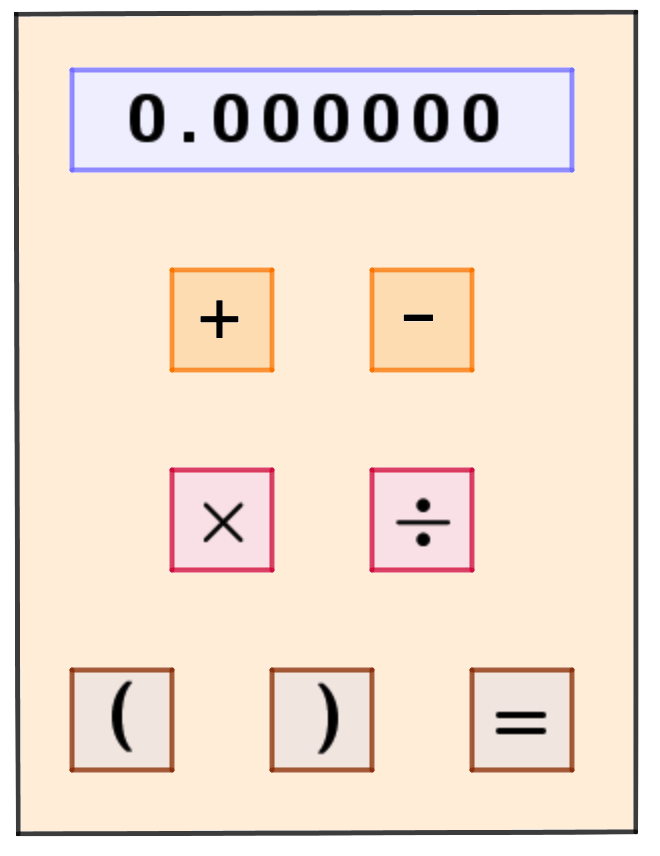
\includegraphics[width=0.35\textwidth]{img-pol/pol01.png}
\end{figure}	
\end{multicols}


El procedimiento usual sería: 

$\ p(0.82)=7.25 \times 0.82 \times 0.82 \times 0.82 - 4.02 \times 0.82 \times 0.82 + 3.19 \times 0.82 - 5.36$	

En total, 6 multiplicaciones, una suma y dos restas, total, $\ 6\times 5+ 3\times 1=33 $ \euro.

\vspace{2mm} Démosle una oportunidad a Ruffini:

\begin{multicols}{2}
\begin{table}[H]
\centering
\begin{tabular}{r|rrrr}
 & 7.25 & -4.02 & 3.19 & -5.36 \\
0.82 & $\downarrow$  & $\boldsymbol{\times}$ & $\boldsymbol{\times}$ & $\boldsymbol{\times}$ \\ \hline
 & 7.25 & $\boldsymbol{+}$ & \multicolumn{1}{r|}{$\boldsymbol{+}$} & $\boldsymbol{+}$ \\ \cline{5-5}
\end{tabular}
\end{table}	

En esta ocasión hemos usado 3 productos y 3 sumas: $\ 3\times 5 + 3\times 1 = 18 $ \euro. Es la opción más económica!
\end{multicols}

Realmente, el método de Ruffini es como sacar factor común:

$p(0.82)=\left[ \left( 7.25 \times 0.82 - 4.02 \right) \times 0.82 + 3.19 \right] \times 0.82 - 5.36 \, , \ $ 3 productos y tres sumas (restas).

\end{myexampleblock}


\vspace{1cm}
\section{Fracciones algebraicas}

\begin{tikzpicture}
	\fill [left color=red!50, right color=teal!50] (0,0) rectangle (3.5,.1);
	\fill [left color=teal!50, right color=blue!50] (3.5,0) rectangle (7.5,.1);
	\end{tikzpicture}
\vspace{0.5cm}



\begin{definition}[ MCM y MCD de polinomios]

\vspace{2mm} El máximo común divisor (MCD) de varios polinomios es el polinomio de mayor grado que es divisor común de todos ellos. 

\vspace{2mm} Para encontrar el MCM de varios polinomios se descomponen estos en factores y se toman los factores comunes elevados a la menor potencia.


\vspace{4mm} El mínimo común multiplo (MCM) de varios polinomios es el polinomio de menor grado que es múltiplo de todos ellos.

\vspace{2mm} Para encontrar el MCM de varios polinomios se descomponen estos en factores y se toman los factores comunes y no comunes elevados a la mayor potencia.
	
\end{definition}

\vspace{4mm}
\begin{miejemplo}

Encuentra el MCM y el MCD de $\ p(x)=x^6-x^2 \ $ y $ \ q(x)=x^3-x^2+x-1$

\vspace{4mm} Primero buscamos la descomposición factorial de ambos polinomios.

\vspace{2mm} $p(x)=x^2(x^4-1)=x^2(x^2-1)(x^2+1)=x^2(x-1)(x+1)(x^2+1)$

\vspace{2mm} Por Ruffin, $\ q(x)=(x-1)(x^2+1)$

\vspace{2mm} $MCD \, \left( p(x),q(x) \right)= (x-1)(x^2+1);\qquad 
MCM \, \left( p(x),q(x) \right)=x^2(x-1)(x+1)(x^2-1)$

\vspace{2mm} \textcolor{gris}{En este caso, al ser $p(x)$ múltiplo de $q(x)$, el MCD es $q(x)$ y el MCM es $p(x)$}
	
\end{miejemplo}

\begin{miejercicio}

Encuentra el MCM y el MCD de los polinomios:

$p(x)=x^2+9x+18;\qquad q(x)=x^2+6x+9;\qquad r(x)=x^2+x-6$

\rule{250pt}{0.1pt}

$p(x)=(x+6)(x+3);\qquad q(x)=(x+3)^2;\qquad r(x)=(x-2)(x+3)$	
 
\vspace{2mm} $MCM(p,q,r)=\, x+3;\qquad $

$MCM(p,q,r)=\, (x-2)(x+3)^2(x+6) \textcolor{gris}{ = x^{4} + 10 \; x^{3} + 21 \; x^{2} - 36 \; x - 108}$
\end{miejercicio}
\vspace{5mm}

\begin{definition}[ Fracción algebraica]

Una \emph{fracción algebraica} es el cociente entre dos polinomios $p(x)$ y $q(x)$, siendo el polinomio del denominador no nulo: $\quad \boldsymbol{\dfrac{p(x)}{q(x)}}$

\vspace{4mm} Al igual que las fracciones de números, dos fracciones algebraicas son \emph{equivalentes} si su producto cruzado coincide.
$\qquad \dfrac{p(x)}{q(x)} \equiv  \dfrac{r(x)}{s(x)} \ \leftrightarrow \ p(x)\cdot s(x)=q(x)\cdot r(x)$

\vspace{4mm} Para \emph{simplificar} una fracción algebraica, se descomponen numerador y denominador en factores y se suprimen los factores comunes a ambos, queda así una fracción equivalente a la original con grados de numerador y denominador menores o iguales.
	
\end{definition}

\begin{miejemplo}

Simplifica la fracción: $\qquad \dfrac{x^3-6x^2+5x+12}{2x^3-7x^2-5x+4}$

\vspace{4mm} Factorizando, por Ruffini, ambos polinomios:

\vspace{2mm} $\dfrac{x^3-6x^2+5x+12}{2x^3-7x^2-5x+4}=
\dfrac { \cancel{(x+1)} (x-3) \bcancel{(x-4)}} { \cancel{(x+1)} \bcancel{(x-4)} (2x-1) }= \dfrac{x-3}{2x-1}$
	
\end{miejemplo}


\begin{theorem}[ Operaciones con fracciones algebraicas]

\begin{itemize}
\item \textbf{Suma y resta}: se procede igual que con las fracciones numéricas, buscando el MCM de los denominadores (para lo que hay que factorizarlos previamente). Al acabar, si es posible, hay que simplificar la fracción algebraica obtenida (en sumas y restas habrá que realizar las operaciones que aparezcan en el numerador, pero el denominador se puede dejar factorizado) .
\item \textbf{Producto y división}: se procede como con las fracciones numéricas. Como al final habrá que simplificar el resultado obtenido y con vista a realizar cálculos más sencillos, es conveniente factorizar previamente las fracciones con que vamos a operar.
\end{itemize}
	
\end{theorem}

\begin{miejemplo}

Realiza la operación: $\quad \dfrac{2}{x-1}-\dfrac{x+3}{x^2-1}+\dfrac{3}{x+1}$
	
\vspace{2mm} $MCM\left( \ x-1, \ x^2-1=(x+1)(x-1),\ x+1 \ \right) \ = \ x^2-1=(x+1)(x-1)$

\vspace{2mm} $\dfrac{2}{x-1}-\dfrac{x+3}{x^2-1}+\dfrac{3}{x+1}= \dfrac
{2(x+1)-(x+3)+3(x-1)}
{(x+1)(x-1)}=
\dfrac{4x-4}{(x+1)(x-1)}= $ 

\vspace{2mm} $=\dfrac {4 \cancel{ (x-1) } }  { \cancel{(x-1)} (x+1) }= \dfrac{4}{x-1} \qquad \to \qquad \dfrac{2}{x-1}-\dfrac{x+3}{x^2-1}+\dfrac{3}{x+1} \ = \  \dfrac{4}{x-1}$
\end{miejemplo}

\begin{miejemplo}

Realiza la operación: $\quad \dfrac{x^2-4}{x^2+4x+4}\, : \, \dfrac{x^2-4x+4}{x^2+2x}$	

\vspace{2mm} Factorizando: $\quad \dfrac{x^2-4}{x^2+4x+4}\, : \, \dfrac{x^2-4x+4}{x^2+2x} = 
\dfrac{(x-2)\cancel{(x+2)}}{(x+2)^{\cancel{2}}}\, : \, \dfrac{(x-2)^2}{x(x+2)}= $

\vspace{2mm} $=\ \dfrac{\cancel{(x-2)}x\bcancel{(x+2)}}{\bcancel{(x+2)}(x-2)^{\cancel{2}}}=\dfrac{x}{x-2} \qquad \to \qquad \dfrac{x^2-4}{x^2+4x+4}\, : \, \dfrac{x^2-4x+4}{x^2+2x} \ = \ \dfrac{x}{x-2}$

\vspace{2mm} 

\vspace{2mm} 
\end{miejemplo}


\begin{figure}[H]
	\centering
	
\includegraphics[width=0.35\textwidth]{img-pol/pol05.png}
\end{figure}




%*****
\begin{miejercicio}

Simplifica: $\quad \dfrac{x^4-8x^2-9}{x^5-6x^3-6x^2-7x-6}$

\rule{250pt}{0.1pt}

\begin{multicols}{2}

$x^4-8x^2-9$

\begin{table}[H]
\centering
\begin{tabular}{r|rrrrr}
 & 1 & 0 & -8 & 0 & -9 \\
3 &  & 3 & 9 & 3 & 9 \\ \hline
 & 1 & 3 & 1 & \multicolumn{1}{r|}{3} & 0 \\ \cline{6-6} 
-3 &  & -3 & 0 & -3 &  \\ \cline{1-5}
 & 1 & 0 & \multicolumn{1}{r|}{1} & 0 &  \\ \cline{5-5}
\end{tabular}
\end{table}

$\nexists x\in \mathbb R \ / \ x^2+1=0$

$(x-3)(x+3)(x^2+1)$

$\qquad$

$\qquad$ %%%%%%

$x^5-6x^3-6x^2-7x-6$

\begin{table}[H]
\centering
\begin{tabular}{r|rrrrrr}
 & 1 & 0 & -6 & -6 & -6 & -6 \\
-1 &  & -1 & 1 & 5 & 1 & 6 \\ \hline
 & 1 & -1 & -5 & -1 & \multicolumn{1}{r|}{-6} & 0 \\ \cline{7-7} 
-2 &  & -2 & 6 & -2 & 6 &  \\ \cline{1-6}
 & 1 & -3 & 1 & \multicolumn{1}{r|}{-3} & 0 &  \\ \cline{6-6}
3 &  & 3 & 0 & 3 &  &  \\ \cline{1-5}
 & 1 & 0 & \multicolumn{1}{r|}{1} & 0 &  &  \\ \cline{5-5}
\end{tabular}
\end{table}

$\nexists x\in \mathbb R \ / \ x^2+1=0$

$(x+1)(x+2)(x-3)(x^2+1)$

\end{multicols}

\vspace{2mm}$\dfrac{x^4-8x^2-9}{x^5-6x^3-6x^2-7x-6}	=\dfrac{(x^2+1)(x+3)(x-3)}{(x^2+1)(x+1)(x+2)(x-3)}=\dfrac{x+3}{(x+2)(x+1)}$
\end{miejercicio}


%*****
\begin{miejercicio}

Calcula: $\quad \dfrac{3x-2}{x^2+x}+\dfrac{4}{x^2-x-2}$

\rule{250pt}{0.1pt}

La factorización de los denominadores es sencilla, 

$\ x^2+x=x(x+1)\ \ $ y $\ \ x^2-x-2=(x+1)(x-2) \quad \to \quad MCM=x(x+1)(x-2)$ 

\vspace{3mm}  $\dfrac{3x-2}{x^2+x}+\dfrac{4}{x^2-x-2}= \dfrac{3x-2}{x(x+1)}+\dfrac{4}{(x+1)(x-2)}=\dfrac{(3x-2)(x-2)+4\, x}{x(x+1)(x-2)}=\dfrac{3x^2-8x+4+4x}{x(x+1)(x+2)}=\dfrac{3x^2-4x+4}{x(x+1)(x+2)}$

\vspace{3mm} Al factorizar el numerador para ver si podemos simplificar, vemos que se trata de un polinomio irreducible. Hemos acabado (no es necesario desarrollar las operaciones que aparecen en el denominador, es mejor dejarlo factorizado).
	
\end{miejercicio}


%*****
\begin{miejercicio}

Calcula: $\quad \left( \dfrac{2x}{x-5}\, : \, \dfrac{3x^2}{x^2-25} \right) \, : \, \dfrac{2x+10}{x}$

\rule{250pt}{0.1pt}

Todos los polinomios que aparecen son fácilmente factorizables: $\ x^2-25=(x-5)(x+5)\ $ y $\ 2x+10=2(x+5)\, , \ $ en este último caso tenemos un polinomio de primer grado que, aún siendo irreducible, es susceptible de sacar factor común (un 2, en este caso).

\vspace{3mm} 
$ \left( \dfrac{2x}{x-5}\, : \, \dfrac{3x^2}{x^2-25} \right) \, : \, \dfrac{2x+10}{x}= \left( \dfrac{2x}{x-5} \, : \, \dfrac{3x^2}{(x-5)(x+5)} \right) \, : \, \dfrac{2(x+5)}{x}= $

\vspace{2mm} $=\dfrac{2\bcancel{x}\cancel{(x-5)}(x+5)}{\cancel{(x-5)}\, 3x^{\bcancel{2}}}\, : \,  \dfrac{2(x+5)}{x}= \dfrac{2(x+5)}{3x}\, : \,  \dfrac{2(x+5)}{x} = \dfrac{\cancel{2}\cancel{(x+5)}\cancel{x}}{3\cancel{x}\, \cancel{2}\cancel{(x+5)}}= \dfrac 1 3$
	
\end{miejercicio}


%*****
\begin{miejercicio}

Calcula: $\quad \left( 4-\dfrac{3x^2}{x^2-1}\right) \cdot \dfrac{x+1}{x^2-4}$

\rule{250pt}{0.1pt}

\vspace{2mm} $\left( 4-\dfrac{3x^2}{x^2-1}\right) \cdot \dfrac{x+1}{x^2-4}=
\left( 	\dfrac 4 1-\dfrac{3x^2}{(x+1)(x-1)}\right) \cdot \dfrac{x+1}{(x+2)(x-2)}=$

\vspace{2mm}
$\dfrac{4(x+1)(x-1)-3x^2}{(x+1)(x-1)} \cdot \dfrac{x+1}{(x+2)(x-2)}=
\dfrac{4x^2-4-3x^2}{(x+1)(x-1)} \cdot \dfrac{x+1}{(x+2)(x-2)}=$

\vspace{2mm} 
$\dfrac{x^2-4}{(x+1)(x-1)} \cdot \dfrac{x+1}{(x+2)(x-2)}=
\dfrac{(x+2)(x-2)}{(x+1)(x-1)} \cdot \dfrac{x+1}{(x+2)(x-2)}=$

\vspace{2mm}
$\dfrac{(x+2)(x-2)(x+1)}{(x+1)(x-1)(x+2)(x-2)} = \dfrac {1}{x-1}$
	
\end{miejercicio}


%*****
\begin{miejercicio}

Calcula: $\quad \left( \dfrac{x}{x^2-3x-4}-\dfrac{2x}{x^2-1}+\dfrac{x^2-6x-4}{x^3-4x^2-x+4} \right) \cdot (x^2-1)$

\rule{250pt}{0.1pt}

Denominadores: 

\vspace{2mm}$\begin{cases}\  x^2-3x-4=(x+1)(x-4) \\ \ 	x^2-1=(x-1)(x+1)\\ \ x^3-4x^2-x+4=(x-1)(x+1)(x-4) \end{cases} \ \to \ \ MCM=\ (x-1)(x+1)(x-4)$

\vspace{4mm}
 $\left( \dfrac{x}{x^2-3x-4}-\dfrac{2x}{x^2-1}+\dfrac{x^2-6x-4}{x^3-4x^2-x+4} \right) \cdot (x^2-1) = $
 
 \vspace{2mm}\begin{small} $= \dfrac{x(x-1)-2x(x-4)+x^2-6x-4}{(x-1)(x+1)(x-4)}  \cdot (x^2-1)= \dfrac{x^2-x-2x^2+8x+x^2-6x-4}{(x-1)(x+1)(x-4)}\cdot (x^2-1)=$ \end{small}
 
 \vspace{2mm} $= \dfrac{x-4}{(x-1)(x+1)(x-4)}\cdot (x^2-1)=\dfrac{1}{(x+1)(x-1)}\cdot (x^2+1)= \dfrac{x^2+1}{(x-1)(x+1)}= 1$	
\end{miejercicio}



%%%%%%%%%%%%%%%%%%%%%%%%%%%%%%%

\section{Ejercicios}

\begin{tikzpicture}
	\fill [left color=red!50, right color=teal!50] (0,0) rectangle (3.5,.1);
	\fill [left color=teal!50, right color=blue!50] (3.5,0) rectangle (7.5,.1);
	\end{tikzpicture}
\vspace{0.5cm}

%************
\begin{mipropuesto}

Calcula: $\quad \left( \, \frac 1 4 x^4+\frac 1 2 x^3+x^2+\frac 5 2 x -\frac 5 4 \, \right) \, : \, \left(\, \frac 1 2 x^2+x-\frac 1 2 \, \right)$
\end{mipropuesto}

\vspace{-8mm}
\begin{flushright}
	\begin{footnotesize} \textcolor{gris}{\rotatebox{180}{ $c(x)= \frac 1 2 x^2 + \frac 5 2 ;\quad r(x)= 0$ }}	\end{footnotesize}
\end{flushright}

%************
\begin{mipropuesto}

Calcula: $\quad \left( \, x^4-\frac 1 2 x^2+\frac 1 3 \, \right) º, : \, \left( \, x+\frac 1 2 \, \right)$ 
\end{mipropuesto}

\vspace{-8mm}
\begin{flushright}
	\begin{footnotesize} \textcolor{gris}{\rotatebox{180}{ $c(x)=x^3-1/2\, x^2-1/4\, x+1/8;\quad r(x)=13/48$ }}	\end{footnotesize}
\end{flushright}


%************
\begin{mipropuesto}

Encontrar el valor de $k$ para que el resto de la división $(x^3-7x^2+3x+k)\, : \, (x^2-x+2)\, $ sea $\, -5x+2$
\end{mipropuesto}

\vspace{-8mm}
\begin{flushright}
	\begin{footnotesize} \textcolor{gris}{\rotatebox{180}{ $k=-10$ }}	\end{footnotesize}
\end{flushright}

%************
\begin{mipropuesto}

Encuentre el valor de $m$ y $n$ para que el resto de la división $(x^4+2x^3+mx+n)\, :\, (x^2+3x-1)$ sea $2x+1$
\end{mipropuesto}

\vspace{-8mm}
\begin{flushright}
	\begin{footnotesize} \textcolor{gris}{\rotatebox{180}{ $m=15,\ \ \ n=-3$ }}	\end{footnotesize}
\end{flushright}


%************
\begin{mipropuesto}

Encuentra el valor de $t$ para que el cociente de la división $(2x^3+\, t \, x^2+6x+1)\, : \, (x^2+5x)$ sea un monomio.
\end{mipropuesto}

\vspace{-8mm}
\begin{flushright}
	\begin{footnotesize} \textcolor{gris}{\rotatebox{180}{ $t=10$ }}	\end{footnotesize}
\end{flushright}



%************
\begin{mipropuesto}

Encuentra el valor de $k$ para que el valor numérico de $p(x)=x^5-x^4+x+3k)$ en $x=2$ sea $5$. ?`Cuál es el resto de dividir $p(x)$ entre $(x-2)$?
\end{mipropuesto}

\vspace{-8mm}
\begin{flushright}
	\begin{footnotesize} \textcolor{gris}{\rotatebox{180}{ $k=-13/3;\ \ \ r(x)=5$ }}	\end{footnotesize}
\end{flushright}


%************
\begin{mipropuesto}

Encuentra los valores de $m$ y $n$ para que $p(x)=x^3-5x^2+mx+n$ sea divisible, a la vez, por $x+1$ y por $x-1$
\end{mipropuesto}

\vspace{-8mm}
\begin{flushright}
	\begin{footnotesize} \textcolor{gris}{\rotatebox{180}{ Sistema dos ecuaciones lineales con dos incógnitas, $\ \ m=-1,\ n=5$ }}	\end{footnotesize}
\end{flushright}

%************
\begin{mipropuesto}

Facroriza los siguientes polinomios:

\begin{multicols}{2}
\begin{enumerate}[a) ]
\item $\ 6x^2-19x-7$
\item $\ x^3+2x^2-20x-40$
\item $\ (4m-2n)x^4-(4m-2n)	$
\item $\ x^5-5x^4+10x^3-10x^2+5x-1$
\end{enumerate}	
\end{multicols}


\end{mipropuesto}



\vspace{-8mm}
\begin{flushright}
	\begin{footnotesize} \textcolor{gris}{\rotatebox{180}{ $a)\ (2x-7)(3x+1);\quad b)\ (x-2)(x+\sqrt{20})(x-\sqrt{20});\quad c)\ 2(2m-n)(x-1)(x+1)(x^2+1);\quad d)\ (x-1)^5$  }}	\end{footnotesize}
\end{flushright}

%************
\begin{mipropuesto}

Sabiendo que $2/5$ es una raíz de $p(x)=20x^3+52x^2+21x-18$, descomponerlo en factores.
\end{mipropuesto}

\vspace{-8mm}
\begin{flushright}
	\begin{footnotesize} \textcolor{gris}{\rotatebox{180}{ Ruffini y ecuación de segundo grado: $\ \ (5x-2)(2x+3)^2$ }}	\end{footnotesize}
\end{flushright}


%************
\begin{mipropuesto}

Encuentra el valor de $a$ y $b$ sabiendo que las siguientes fracciones algebraicas son equivalentes:
$\qquad  \dfrac{x^2-3x-10}{x^2+5x+a};\qquad \dfrac{x-b}{x+3}$
\end{mipropuesto}

\vspace{-8mm}
\begin{flushright}
	\begin{footnotesize} \textcolor{gris}{\rotatebox{180}{ $a=6;\ \ b=5$ }}	\end{footnotesize}
\end{flushright}

%************
\begin{mipropuesto}

Simplifica las siguientes fracciones algebraicas:

\begin{multicols}{2}
\begin{enumerate}[a) ]
\item $\dfrac{x^2+3x-4}{x^2+4x}$
\item $\dfrac{2x^3-2}{x^3-x^2-x-2}$
\item $\dfrac{x^4-2x^3+x^2-2x}{x^2-4}$
\item $\dfrac{x^5-x^2}{x^4+x^3+x^2}$	
\end{enumerate}	
\end{multicols}
\vspace{1mm}
\end{mipropuesto}

\vspace{-8mm}
\begin{flushright}
	\begin{footnotesize} \textcolor{gris}{\rotatebox{180}{ $a)\ \dfrac{x-1}{x};\quad b)\ \ \dfrac{2x-2}{x-2};\quad c)\ \ \dfrac{x^3+x}{x+2};\quad d)\ \ x-1 $ }}	\end{footnotesize}
\end{flushright}

%************
\begin{mipropuesto}

Escribe una fracción de numerador $\, 20x-5\, $ que sea equivalente a $\dfrac{5}{3x+1}$
\end{mipropuesto}

\vspace{-8mm}
\begin{flushright}
	\begin{footnotesize} \textcolor{gris}{\rotatebox{180}{ $\dfrac{20x-5}{12x^2+x-1}$ }}	\end{footnotesize}
\end{flushright}


%************
\begin{mipropuesto}

Realiza las siguientes operaciones:

\begin{multicols}{2}
\begin{enumerate}[a) ]
\item $\dfrac{1-x^2}{x^2-4x}+\dfrac{3x-x^2}{4x-x^2}+\dfrac{x^2-x-1}{x^2-4x}$
\item $\dfrac{x-4}{x+2}+\dfrac{x-1}{x+3}$
\item $\dfrac{x-2}{x-1}+\dfrac{x-1}{x+1}$
\item $\dfrac{1}{2x-4}+\dfrac{x-3}{x+2}+\dfrac{x-x^2}{x^2-4}$	
\item $\dfrac{3}{x+3}-\dfrac{1}{x+2}-\dfrac{x}{x^2+5x+6}$
\item $\dfrac{x-1}{x-3}+\dfrac{x+4}{x+2}-\dfrac{2x^2+3x-12}{x^2-x-6}$
\end{enumerate}	
\end{multicols}
\vspace{1mm}
\end{mipropuesto}

\vspace{-8mm}
\begin{flushright}
	\begin{footnotesize} \textcolor{gris}{\rotatebox{180}{ $a)\ -1;\ \ \ b)\ \dfrac{2x^2-14}{x^2+5x+6};\ \ \ c)\ \dfrac{2x^2-3x-1}{x^2-1}; \ \ \ d)\ \dfrac{x-10}{2x^2-8};\ \ \ e)\ \dfrac{1}{x+2};\ \ \ f)\ \dfrac{1}{3-x}$ }}	\end{footnotesize}
\end{flushright}

%************
\begin{mipropuesto}

Realiza las siguientes operaciones:

\begin{multicols}{2}
\begin{enumerate}[a) ]
\item $\dfrac{x^2+2x+1}{x-3}\cdot \dfrac{x^2+x-12}{x^2-1}$
\item $\dfrac{x^2-2x-3}{x^2-5x}\cdot \dfrac{x^2-4x-5}{x^2-4x+3}$
\item $\dfrac{x+2}{x^2+4x+4}\, : \, \dfrac{x^2-4}{x^3+8}$
\item $\left( \dfrac{x+5}{x-3} -1\right)\cdot \left( \dfrac{4-x}{x-2}+1\right)$
\end{enumerate}	
\end{multicols}
\vspace{1mm}	
\end{mipropuesto}

\vspace{-8mm}
\begin{flushright}
	\begin{footnotesize} \textcolor{gris}{\rotatebox{180}{ $a)\ \dfrac{x^2+5x+4}{x-1};\ \ \ b)\ \dfrac{x*2+2x+1}{x^2-x};\ \ \ c)\ \dfrac{x^2-2x+4}{x^2-4};\ \ \ d)\ \dfrac{16}{x^2-5x+6}$ }}	\end{footnotesize}
\end{flushright}

%************
\begin{mipropuesto}

Calcula:
$\qquad \left( \, x+1\, + \, \dfrac{x^3}{x-x^2} \, \right) \, : \, \left( \, 1\, -\, \dfrac{1}{x+1} \cdot \dfrac{2x}{1-x^2} \, \right)$
\end{mipropuesto}

\vspace{-8mm}
\begin{flushright}
	\begin{footnotesize} \textcolor{gris}{\rotatebox{180}{ Simplifica a medida que calculas $\quad \dfrac{1}{2-x}$ }}	\end{footnotesize}
\end{flushright}


%************
\begin{mipropuesto}

Calcula: $\qquad a)\ \ \dfrac{x-\dfrac{x}{x+1}}{x+\dfrac{x}{x-1}} \, ; \qquad \qquad b)\ \ \dfrac{1-\dfrac{1+x^2}{1-x^2}}{1+\dfrac{1+x^2}{1-x^2}}$
\end{mipropuesto}

\vspace{-8mm}
\begin{flushright}
	\begin{footnotesize} \textcolor{gris}{\rotatebox{180}{ $a)\ \dfrac{x-1}{x+1};\ \ \ b)\ -x^2$ }}	\end{footnotesize}
\end{flushright}

%%%%%%%%%%%%%%%%%%%%%%%%%%%%%%%%%%%%


\newpage

$\quad$

$\quad$


\begin{adjustwidth}{50pt}{250pt}
\begin{cuadro-naranja}
\textbf{\huge{Problemas $\boldsymbol{+}$}}\normalsize{$\, $}
\end{cuadro-naranja}	
\end{adjustwidth}

\vspace{5mm}
\begin{enumerate}[\textbf{P$\boldsymbol +$} 1. ]
\item	Factoriza el polinomio: $\ \ (x+3)^3-(x+2)^3-(x+1)^3-x^3$

\vspace{-6mm}
\begin{flushright}
\begin{footnotesize} \textcolor{gris}{\rotatebox{180}{ $2(x-3)(x^2+3x+3)$ }}	\end{footnotesize}
\end{flushright}


\item	Si $6$ es raíz de $p(x)=x^2-2x+1$, ?`cuál es el valor de $a$?

\vspace{-6mm}
\begin{flushright}
\begin{footnotesize} \textcolor{gris}{\rotatebox{180}{ -4 }}	\end{footnotesize}
\end{flushright}


\item	$x^2-n^2x+2n$ tiene dos raíces distintas, si una es $n=2$, ?`cuál es la otra?

\vspace{-6mm}
\begin{flushright}
\begin{footnotesize} \textcolor{gris}{\rotatebox{180}{ -1 }}	\end{footnotesize}
\end{flushright}

%
\item	Sea un polinomio tal que $\ p(x^2+1)= x^4+4x^2\, , \ $ determina $p(x^2-1)$

\vspace{-6mm}
\begin{flushright}
\begin{footnotesize} \textcolor{gris}{\rotatebox{180}{a la hipótesis ($x^4+4x^2$). Identifica coeficientes. Luego, calcula $p(x^2-1$. $\quad$ sol: $p(x^2-1)=x^4-4$}}	\end{footnotesize}
\end{flushright}
\vspace{-8mm}
\begin{flushright}
\begin{footnotesize} \textcolor{gris}{\rotatebox{180}{ $p(x)$ ha de ser un polinomio de segundo grado, $p(x)=ax^2+bx+c$. Calcula $p(x^2+1)$ e iguala  }}	\end{footnotesize}
\end{flushright}


%
\item	Al dividir $p(x)$ entre $(x-1)$ el resto es $-8$, si lo dividimos por $(x+2)$ el resto es $25$. ?`Cuál es el resto de dividir a $p(x)$ entre $x^2+x-2\,$?

\vspace{-6mm}
\begin{flushright}
\begin{footnotesize} \textcolor{gris}{\rotatebox{180}{ $p(1)=-8;\ p(-2)=25;\ x^2+x-2=(x-1)(x+2)$  El resto de dividir $p(x)$ por $x^2+x-2$ será }}	\end{footnotesize}
\end{flushright}
\vspace{-8mm}
\begin{flushright}
\begin{footnotesize} \textcolor{gris}{\rotatebox{180}{un polinomio de primer grado, $mx+n$, luego $p(x)=c(x)(x-1)(x+2)+(mx+n)$ }}	\end{footnotesize}
\end{flushright}
\vspace{-8mm}
\begin{flushright}
\begin{footnotesize} \textcolor{gris}{\rotatebox{180}{ Impón tus condiciones y la solución es: $\ -11x+3$}}	\end{footnotesize}
\end{flushright}
 
\end{enumerate}



%%%%%%%%%%%%%%%%%%%%%%%%%%%%%%%%%%%%
\newpage
\section{Resumen del tema}

\begin{tikzpicture}
	\fill [left color=red!50, right color=teal!50] (0,0) rectangle (3.5,.1);
	\fill [left color=teal!50, right color=blue!50] (3.5,0) rectangle (7.5,.1);
	\end{tikzpicture}
\vspace{1cm}


\begin{myblock}{Resumen: \emph{``Polinomios y fracciones algebraicas''}}

\underline{Teorema del resto}:  $a$ es raíz de $p(x)$ si $p(a)=0 \ \Rightarrow \ p(x) $ es divisible por $\ x-a$ .

\vspace{2mm}
--- Los polinomios de primer grado son irreducibles.

--- Los polinomios de segundo grado con soluciones reales $x_1$ y $x_2$ se pueden factorizar como $a(x-x_1)(x-x_2)\, . \ $ Si no hay soluciones reales, el polinomio es primo.

\vspace{5mm} Si $p(x)$ tiene coeficientes enteros $\ \Rightarrow $

\begin{itemize}
\item Candidatos a raíces enteras: 	$\ \pm $ divisores del término independiente.
\item Candidatos a raíces racionales: 	$\ \pm $ divisores del término independiente, dividido por divisores del término dominante.
\end{itemize}


\vspace{3mm}
\begin{small}
Si el polinomio tiene coeficientes enteros, el \textbf{procedimiento} a seguir para factorizarlo será el siguiente:

\begin{enumerate}
\vspace{-2mm}\item Encontramos los divisores del término independiente. Si no tuviese término independiente sacaríamos factor común y seguiríamos intentando factorizar el resultado.

\vspace{-2mm}\item Comprobamos si son raíces del polinomio, comenzando
por el más pequeño.

\vspace{-2mm}\item Con el primero que encontremos aplicamos la regla de
Ruffini.

\vspace{-2mm}\item Tomamos el cociente que hayamos obtenido y
repetimos el proceso empezando a probar con la misma
raíz obtenida anteriormente.

\vspace{-2mm}\item Si un divisor del término independiente no es raíz en un
paso, tampoco lo será en el siguiente. Puede que haya raíces repetidas (dobles, triples, etc.); por lo tanto, si una raíz lo es en un paso, también lo puede ser en el siguiente.

\vspace{-2mm}\item Cuando tengamos un cociente de grado 2, podemos resolver la ecuación correspondiente de 2o grado. Es la única opción que tenemos si el polinomio tiene raíces reales no enteras (racionales o irracionales). 

$ax^2+bx+c=0 \to x=x_1 \vee x=x_2 \ \Rightarrow \ \boldsymbol{ax^2+bx+c=a(x-x_1)(x-x_2)}$

\vspace{-2mm}\item Finalmente escribimos la descomposición en producto de factores del polinomio.
\end{enumerate}
El \emph{teorema fundamental del álgebra} asegura que un polinomio de grado $n$ tiene, a lo sumo, $n$ raíces reales.

También se pueden usar los \emph{productos notables} para la factorización de polinomios. 
\end{small}	
\end{myblock}





\begin{comment}
%%%%%%%%%%%%%%%%%%%%%%%%%%%%%%%%%%%. SECCIONES
\begin{figure}[H]
	\centering
	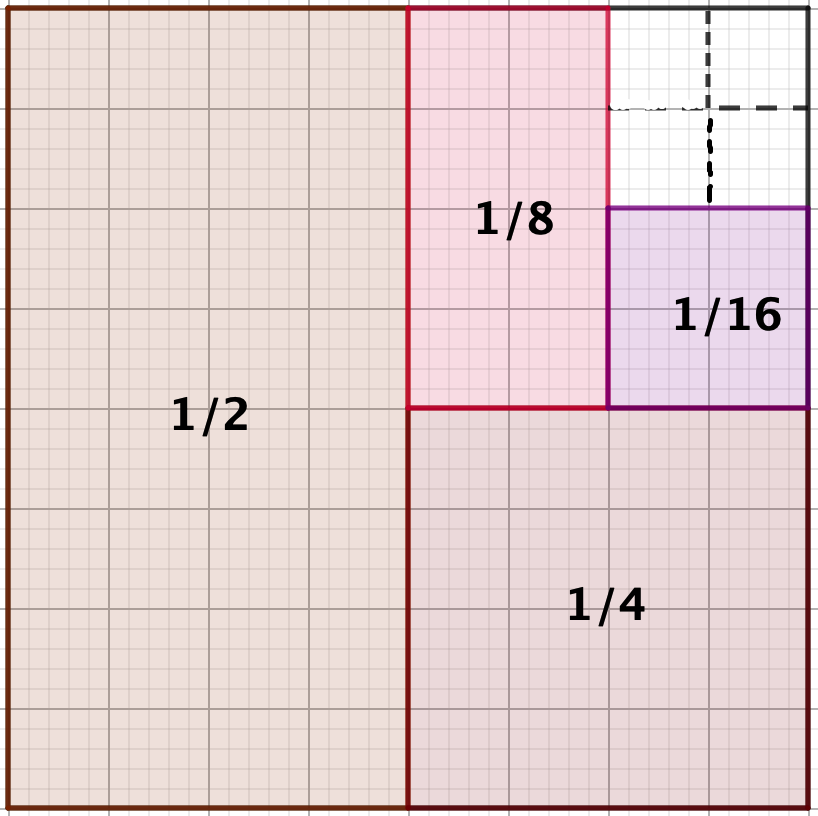
\includegraphics[width=0.25\textwidth]{img-suc/suc03.png}
\end{figure}



\chapter{texto}

\begin{tikzpicture}
	\fill [left color=red!50, right color=teal!50] (0,0) rectangle (6.5,.2);
	\fill [left color=teal!50, right color=blue!50] (6.5,0) rectangle (11.5,.2);
	\end{tikzpicture}

\vspace{1cm}
\section{texto}

\begin{tikzpicture}
	\fill [left color=red!50, right color=teal!50] (0,0) rectangle (3.5,.1);
	\fill [left color=teal!50, right color=blue!50] (3.5,0) rectangle (7.5,.1);
	\end{tikzpicture}
\vspace{0.5cm}

\subsection{texto}

\begin{tikzpicture}
	\fill [left color=red!50, right color=teal!50] (0,0) rectangle (3.5,.01);
	\fill [left color=teal!50, right color=blue!50] (3.5,0) rectangle (7.5,.01);
	\end{tikzpicture}
\vspace{0.5cm}


%%%%%%%%%%%%%%%%%%%%%%%%%%%%%%%%%%%. \begin{ ------>. 
detsacado;  cuadro-naranja;  cuadro-gris;  miejercicio (solución extensa);  mipropuesto (solución corta y fuera del cuadro) \theomen  \definition

%%%%%%%%%%%%%%%%%%%%%%%%%%%%%%%%%%%. CURIOSIDAD
\vspace{1cm}
\color{ForestGreen!80}
\rule{250pt}{0.2pt}
Texto
\vspace{-8mm}
\begin{flushright}
\rule{250pt}{0.2pt}		
\end{flushright}	
\color{black}
\end{comment}